% id: 49-23
% book: 베이직쎈 확률과 통계 · 03 확률의 뜻과 활용
% section: 유형 028 조합을 이용하는 확률
% figure: tikz:fig-49-23
% answer: 
% answer_source: 
% variant_level: 0 (원본 전사)
% 이 파일은 build.mjs 가 items.json 에서 만든다. 고칠 때는 items.json 을 고친다.
\smash{\raisebox{1.5mm}{\dmkichul{베이직쎈 확률과 통계 49쪽 23번}}}
\noindent\begin{minipage}[t]{0.58\linewidth}\vspace{0pt}\raggedright 오른쪽 그림과 같이 원 위에 같은 간격으로 놓인 8개의 점 중에서 임의로 3개의 점을 택하여 그 3개의 점을 꼭짓점으로 하는 삼각형을 만들 때, 다음을 구하시오.\end{minipage}\hfill\begin{minipage}[t]{0.4\linewidth}\vspace{0pt}\centering \resizebox{\ifdim\width>\linewidth\linewidth\else\width\fi}{!}{% 유형 028 49-23(인쇄 49쪽) — 원 위에 같은 간격으로 놓인 8개의 점. 스캔 화질이 낮아 TikZ 로 다시 그림.
% 원문대로 점만 찍고 지름·삼각형은 그리지 않는다(직각삼각형의 개수가 그림에서 읽히지 않게). 라벨은 원문에 없다.
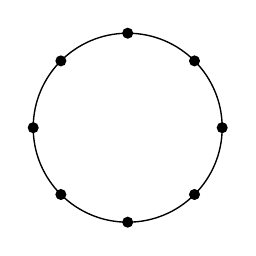
\begin{tikzpicture}[scale=1, line width=0.5pt]
  \draw (0,0) circle (1.2);
  \foreach \a in {0,45,...,315} { \fill (\a:1.2) circle (2pt); }
\end{tikzpicture}
}\end{minipage}\par
\dmsubprob{1} 만들 수 있는 삼각형의 개수
\dmsubprob{2} 만들 수 있는 직각삼각형의 개수
\dmsubprob{3} 만든 삼각형이 직각삼각형일 확률
